%%%%%%%%%%%%%%%%%%%%%%%%%%%%%%%%%%%%%%
% LaTeX poster template
% Created by Nathaniel Johnston
% August 2009
% http://www.nathanieljohnston.com/2009/08/latex-poster-template/
%%%%%%%%%%%%%%%%%%%%%%%%%%%%%%%%%%%%%%

\documentclass[final]{beamer}
\usepackage[scale=1.24]{beamerposter}
\usepackage{graphicx}			% allows us to import images

%-----------------------------------------------------------
% Define the column width and poster size
% To set effective sepwid, onecolwid and twocolwid values, first choose how many columns you want and how much separation you want between columns
% The separation I chose is 0.024 and I want 4 columns
% Then set onecolwid to be (1-(4+1)*0.024)/4 = 0.22
% Set twocolwid to be 2*onecolwid + sepwid = 0.464
%-----------------------------------------------------------

\newlength{\sepwid}
\newlength{\onecolwid}
\newlength{\twocolwid}
\newlength{\threecolwid}
\setlength{\paperwidth}{48in}
\setlength{\paperheight}{36in}
\setlength{\sepwid}{0.024\paperwidth}
\setlength{\onecolwid}{0.22\paperwidth}
\setlength{\twocolwid}{0.464\paperwidth}
\setlength{\threecolwid}{0.708\paperwidth}
\setlength{\topmargin}{-0.5in}
\usetheme{confposter}
\usepackage{exscale}
\usepackage{verbatim}
\usepackage{fancyvrb}

%-----------------------------------------------------------
% The next part fixes a problem with figure numbering. Thanks Nishan!
% When including a figure in your poster, be sure that the commands are typed in the following order:
% \begin{figure}
% \includegraphics[...]{...}
% \caption{...}
% \end{figure}
% That is, put the \caption after the \includegraphics
%-----------------------------------------------------------

\usecaptiontemplate{
\small
\structure{\insertcaptionname~\insertcaptionnumber:}
\insertcaption}

%-----------------------------------------------------------
% Define colours (see beamerthemeconfposter.sty to change these colour definitions)
%-----------------------------------------------------------

\setbeamercolor{block title}{fg=ngreen,bg=white}
\setbeamercolor{block body}{fg=black,bg=white}
\setbeamercolor{block alerted title}{fg=white,bg=dblue!70}
\setbeamercolor{block alerted body}{fg=black,bg=dblue!10}

%-----------------------------------------------------------
% Name and authors of poster/paper/research
%-----------------------------------------------------------

\title{Part Handling in qooxdoo 3}
\institute{Thomas Herchenr\"oder, 1\&1 Internet AG (\today)}

%-----------------------------------------------------------
% Start the poster itself
%-----------------------------------------------------------

\begin{document}
\begin{frame}[t]
  \begin{columns}[t]												% the [t] option aligns the column's content at the top
    \begin{column}{\sepwid}\end{column}			% empty spacer column
    \begin{column}{\onecolwid}
      \begin{block}{Parts}
        \textit{Parts} are a means to \textit{logically} partition a qooxdoo
        application, so that those parts can be loaded \textit{incrementally}
        and \textit{on demand}. Parts are defined through
        configuration, and the \textit{Generator} 
        distributes class code and resource information across multiple script
        files that are then retrieved via HTTP. The aim is to avoid loading
        of unnecessary code and data into the browser.
      \end{block}
      \vskip2ex
      \begin{block}{Concepts}
        The Generator collects \textit{class} code into
        \textit{scripts} (.js files). Scripts are grouped into
        \textit{packages}. Scripts of the same package are always loaded
        together. Each \textit{part} is
        implemented by a collection of packages, each package might be required
        by multiple parts. qooxdoo's \textit{PartLoader} loads all packages for
        a part that has been required, but have not been loaded yet.
        \begin{figure}
          \begin{center}
            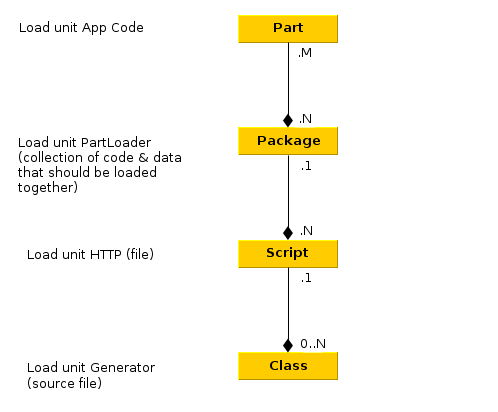
\includegraphics[width=10in]{g_relations.png} \\
            \caption{Relations between parts, packages, scripts and classes}
            \label{fig:corrSubsys}
          \end{center}
        \end{figure}
      \end{block}


      \begin{block}{Configuring Parts}
        Specifying the \textit{include} key of the part definitions.
        (\textit{``include list''} means all entries after glob expansion.)
        \begin{itemize}
          \item the \textit{boot} part should have \textit{the same} include definition
            as the application
          \item include lists must be \textit{free of overlaps}
          \item \textit{load dependencies} of one part must not be in include lists of
            other parts
        \end{itemize}
      \end{block}

      \vskip2ex
    \end{column}

    % column 2

    \begin{column}{\sepwid}\end{column}			% empty spacer column

    \begin{column}{\twocolwid}  % 2-column middle
    \begin{columns}[t,totalwidth=\twocolwid] % split in 2
    \begin{column}{\onecolwid}
      \begin{block}{}
        \begin{itemize}
          \item don't define include lists along \textit{physically boundaries} (name
            spaces, libraries, ...)
          \item don't define parts with \textit{framework classes}
        \end{itemize}
      \end{block}

      \begin{block}{2-Phase Package Calculation}
        Assign classes to packages in a 2-step process:
        \begin{itemize}
          \item \textbf{equivalence sets} group all classes that are required by the
            same set of parts
          \item \textbf{merging} (or collapsing) resolve smaller packages into
            larger ones
            \begin{itemize}
              \item by order (\textit{collapse groups})
              \item by size
            \end{itemize}
        \end{itemize}
      \end{block}
    \end{column}

    \begin{column}{\sepwid}\end{column}			% empty spacer column
    \begin{column}{\onecolwid}
      \begin{block}{Equivalence Sets}
        To construct the equivalence sets for the classes:
        \begin{itemize}\justifying
          \item \textbf{part class list}: calculate the class list starting from
            part's \textit{include}, skipping other seeds
          \item \textbf{class labeling}: assigne each class the parts which require it
          \item \textbf{classify}: group classes that are required by the same parts
        \end{itemize}
        If $N$ is the number of defined parts then\\
        \begin{center}
          $ max(count(equivalence\_sets(N))) = 2^{N} - 1 $
        \end{center}
      \end{block}
    \end{column}

    \end{columns}

    % center image

    \begin{figure}   % ACTUAL two-column-wide column
      \begin{center}
        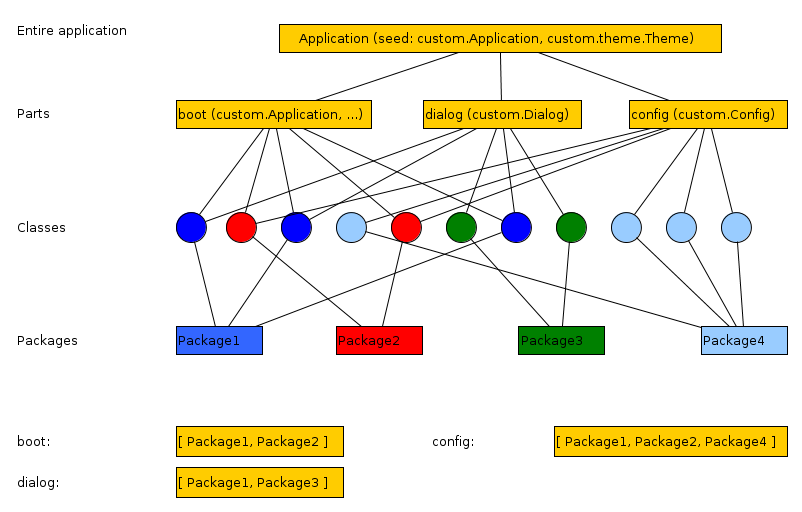
\includegraphics[width=20in]{g_part_layers.png} \\
        \caption{Mapping parts to classes, and classes to packages}
        \label{fig:corrSubsys}
      \end{center}
    \end{figure}

    % middle bottom

    \begin{columns}[t,totalwidth=\twocolwid]
    \begin{column}{\onecolwid}
      \begin{block}{Part Assertions}
        \begin{itemize}
          \item parts are \textbf{lazy run deps}
          \item each part is \textbf{self-contained} \textit{wrt} load deps 
          \item this is also true for \textit{expected-load-order}, parts
            can be loaded out-of-order
          \item every class is only loaded \textbf{once}
          \item classes are \textbf{load-ordered} within a package, packages are
            load-ordered within a part
        \end{itemize}
      \end{block}

    \end{column}

    \begin{column}{\onecolwid}
      \begin{block}{References}
        \small{\begin{thebibliography}{99}
          \bibitem P``Parts and Packages Overview'', qooxdoo Manual, http://bit.ly/1hL6cqU
          \bibitem U``Using Parts'', qooxdoo Manual, http://bit.ly/17y8MMH
          \bibitem G``Generator Config Keys - packages'', qooxdoo Manual, http://bit.ly/177sNXW 
          \bibitem qqx.io.PartLoader, qooxdoo API, http://bit.ly/1cvQM2Q 
        \end{thebibliography}}
      \end{block}

    \end{column}

    \end{columns}
    \end{column}  % 2-column middle

    % column 4

    \begin{column}{\sepwid}\end{column}			% empty spacer column

    \begin{column}{\onecolwid}

      \begin{block}{Package Dependencies}
        Classes $c_1, c_2$, packages $p_1, p_2$, part $P_1$, then
        \begin{itemize}
          \item $if\ c_1 \in p_1\ and\ c_2 \in p_2\ and\ depends(c_1,c_2) \Rightarrow
            depends(p_1,p_2)$
          \item $ordered(P_1) \Leftrightarrow ordered(Packages(P_1))\ and\ 
            \forall P \in Packages(P_1): ordered(P)$
        \end{itemize}
      \end{block}

      \begin{block}{Package Merging}
        Let $p_1$ be package for merging into $p_2$, $Parts(x)$ be
        the set of parts a package is used in, $Deps(x)$ be the load depedencies of
        a class or package, then
        \begin{itemize}
          \item Classes($p_1$) go into $p_2$, $p_1$ is removed
          \item $Parts(p_1) \subset Parts(p_2)$  [$p_2$ must at least be used where $p_1$ is
            used]
          \item after the merge: $\forall P \in Parts(p_2): ordered(P)$
          \item $\forall P \in Parts(p_2): Deps(p_1) \subset P$
            [dependencies of $p_1$ must be fullfilled wherever $p_2$ is used]
          \item \textit{expected-load-order} more aggressive merging
          \item classes will be loaded where not needed
          \item \textit{parts verifier} checks these constraints
        \end{itemize}
        \begin{figure}
          \begin{center}
            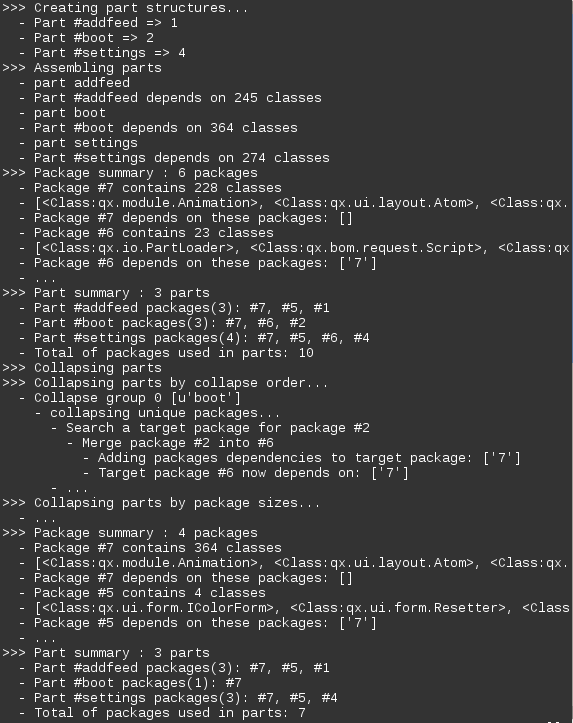
\includegraphics[width=\onecolwid]{g_parts_log.png}
            \caption{Part creation verbose output (excerpt)}
            \label{fig:corrSubsys}
          \end{center}
        \end{figure}
      \end{block}

    \end{column}

  \end{columns}
\end{frame}
\end{document}
